\renewcommand{\theequation}{\theenumi}
\begin{enumerate}[label=\arabic*.,ref=\thesubsection.\theenumi]
\numberwithin{equation}{enumi}
\item Total n0 of student = 90
\\
no of students who obtained marks less than $20\%= 7$
\\
assume that $P(X<20)$ is the probability of the students obtained less than 20$\%$ marks 
\begin{align}
	P\left(X<20\right) &= \frac{7}{90}
	\\
	&=0.07
\end{align}
\\
\item no of the students obtained 60-70 marks = 15
\\
no of the student obtained 70 above marks = 8
\\
$P(X \geq 60)$= probability of a student obtained 60 0r above marks 
\begin{align}
P\left(X \geq 60\right) &= \frac{15 + 8}{90}
\\
&= 0.256
\end{align}
\begin{lstlisting}
codes/prob/prob5.py
\end{lstlisting}
\begin{figure}[!ht]
	\centering
	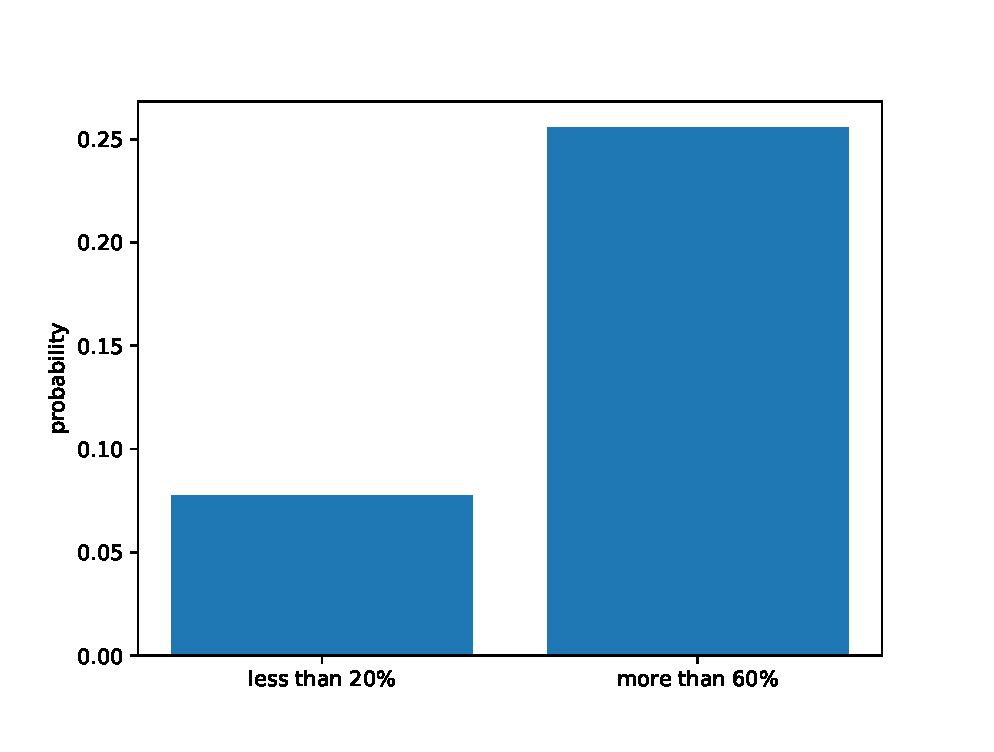
\includegraphics[width=\columnwidth]{./figures/prob/prob5.eps}
	\caption{probability of marks of students }
	\label{fig:bt5}
	\begin{lstlisting}
	figs/prob/prob5.py
	\end{lstlisting}
\end{figure}
\end{enumerate}